%%%%%%%%%%%%%%%%%%%%%%%%%%%%%%%%%%%%%%%%%
% Beamer Presentation
% LaTeX Template
% Version 1.0 (10/11/12)
%
% This template has been downloaded from:
% http://www.LaTeXTemplates.com
%
% License:
% CC BY-NC-SA 3.0 (http://creativecommons.org/licenses/by-nc-sa/3.0/)
%
%%%%%%%%%%%%%%%%%%%%%%%%%%%%%%%%%%%%%%%%%

%----------------------------------------------------------------------------------------
%	PACKAGES AND THEMES
%----------------------------------------------------------------------------------------

\documentclass{beamer}

\mode<presentation> {

% The Beamer class comes with a number of default slide themes
% which change the colors and layouts of slides. Below this is a list
% of all the themes, uncomment each in turn to see what they look like.


% \usetheme{default}
% \usetheme{AnnArbor}
% \usetheme{Antibes}
% \usetheme{Bergen}
% \usetheme{Berkeley} % neat
% \usetheme{Berlin} % nice
% \usetheme{Boadilla}
% \usetheme{CambridgeUS} %nice colors
% \usetheme{Copenhagen} % neat
% \usetheme{Darmstadt} % simple and neat
% \usetheme{Dresden} %nice and neat
% \usetheme{Frankfurt} % clean and -neat
% \usetheme{Goettingen} % clean and -neat
% \usetheme{Hannover} % neat and clean
% \usetheme{Ilmenau} % nice but dangerous layout
% \usetheme{JuanLesPins} % nice
% \usetheme{Luebeck} % clean and nice
% \usetheme{Malmoe} % same
% \usetheme{Madrid} % simple
\usetheme{Marburg} % beautiful simple and neat
% \usetheme{Montpellier} % very simple
% \usetheme{PaloAlto} % clear and nice and neat
% \usetheme{Pittsburgh}
% \usetheme{Rochester} %simple and not neat 
% \usetheme{Singapore} %meh
% \usetheme{Szeged} % a bit ugly 
% \usetheme{Warsaw} % clear and neat

% As well as themes, the Beamer class has a number of color themes
% for any slide theme. Uncomment each of these in turn to see how it
% changes the colors of your current slide theme.

% \usecolortheme{albatross}
% \usecolortheme{beaver}
% \usecolortheme{beetle}
% \usecolortheme{crane} % nice
\usecolortheme{dolphin} % very nice
% \usecolortheme{dove}
% \usecolortheme{fly}
% \usecolortheme{lily} % clean
% \usecolortheme{orchid} % clean
% \usecolortheme{rose}
% \usecolortheme{seagull}
% \usecolortheme{seahorse}
% \usecolortheme{whale} % clean
% \usecolortheme{wolverine}

% \setbeamertemplate{footline} % To remove the footer line in all slides uncomment this line
\setbeamertemplate{footline}[page number] % To replace the footer line in all slides with a simple slide count uncomment this line

\setbeamertemplate{navigation symbols}{} % To remove the navigation symbols from the bottom of all slides uncomment this line
}

\usepackage{graphicx} % Allows including images
\usepackage{booktabs} % Allows the use of \toprule, \midrule and \bottomrule in tables

%----------------------------------------------------------------------------------------
%	TITLE PAGE
%----------------------------------------------------------------------------------------

\title[Présentation]{Séance 2} % The short title appears at the bottom of every slide, the full title is only on the title page

\author{A. Cercy} % Your name
\institute[] % Your institution as it will appear on the bottom of every slide, may be shorthand to save space
{
Collège Pablo Neruda
}
% \date{\today} % Date, can be changed to a custom date
\date{} % Date, can be changed to a custom date

\begin{document}

\begin{frame}
\titlepage % Print the title page as the first slide
\end{frame}

\begin{frame}
\frametitle{Plan} % Table of contents slide, comment this block out to remove it
\tableofcontents % Throughout your presentation, if you choose to use \section{} and \subsection{} commands, these will automatically be printed on this slide as an overview of your presentation
\end{frame}
%%-------------------------------------------------------------

\begin{frame}
    \frametitle{Pour commencer}
    \centerline{Se mettre à sa place habituelle et rester debout.}
\end{frame}


\section{Nouveau chapitre}
\begin{frame}
\frametitle{Nouveau chapitre}
Prendre la page blanche suivante du cahier et tout en haut, en rouge et souligné, écrire "Chapitre 1 : Être au courant" puis \textbf{laisser le reste de la page blanche}.
\end{frame}


\section{L'activité du jour}
\begin{frame}
\frametitle{L'activité du jour}
Sur la page suivante, coller l'activité 1 : Perdus dans le noir
\end{frame}


\section{Lecture de l'activité}
\begin{frame}
\frametitle{Lecture de l'activité}
Nous lisons l'activité ensemble.
\end{frame}


\section{Matériel et question 1}
\begin{frame}
\frametitle{Matériel et question 1}
Question 1 : Par binôme, réaliser un circuit électrique pour allumer l’ampoule. Vous disposez d’une
pile cylindrique, d’un fil et d’une ampoule...
\end{frame}


\section{Question 2}
\begin{frame}
\frametitle{Question 2}

(a) Dessinez tous les circuits possibles où la lampe s’allume.
Il faut qu'on voit très précisément l'ampoule et la pile et leur différentes parties.

\vspace{10pt}
\textbf{\textit{Avant les dessins, écrivez "Question 2 (a)" sur votre cahier:}}

\end{frame}



\section{Question 2 suite}
\begin{frame}
\frametitle{Question 2 suite}
(b) Même travail mais avec une pile plate (qu’il faut aller chercher) qui remplace la pile cylindrique.

\vspace{5pt}
(c) Dessinez  une ampoule avec le filament à l’intérieur de l’ampoule.
\end{frame}



\section{Question 2 suite}
\begin{frame}
\frametitle{Question 2 suite}
Question 2 :

(d)Vous venez de réaliser un circuit électrique pour allumer la lampe ! 

Quelles sont les conditions pour que la lampe s’allume, autrement dit, comment définiriez vous un circuit électrique ?
\end{frame}


\section{Correction}
\begin{frame}
    \frametitle{Correction}
    Il faut participer à la correction et la recopier sur l'activité.
\end{frame}

\section{Cours}
    \begin{frame}
    \frametitle{Cours}
    Il faut recopier le cours dans \textbf{\textit{En dessous du début du chapitre}}
    
\end{frame}


% \subsection{L'important c'est de trouver son chemin à soi}
% \begin{frame}
% \frametitle{L'important c'est de trouver son chemin à soi}
% \begin{columns}[c] % The "c" option specifies centered vertical alignment while the "t" option is used for top vertical alignment

% \column{.45\textwidth} % Left column and width
% \textbf{Parfois}
% la physique chimie ce n'est pas le plus urgent dans l'immédiat,
% parfois on va mal, on est fatigué.e, on a d'autres problèmes

% \column{.5\textwidth} % Right column and width
% C'est tout à fait normal, c'est pour ça que c'est 
% si important de se respecter les uns les autres

% \end{columns}

% \end{frame}

% \section{We need you}
% \begin{frame}
% \frametitle{We need you}
% \begin{figure}
%     
\includegraphics[width=0.8\linewidth]{we_need_you.jpg}
% \end{figure}
% \end{frame}

% \begin{frame}
%     \frametitle{Une classe accueillante pour tous}
%     \begin{itemize}
%         \item Peu importe son genre (garçon ou fille)
%         \item Peu importe sa sexualité
%         \item Peu importe son style etc
%     \end{itemize}
% \end{frame}


% \begin{frame}
% \frametitle{M'aider à orienter mon cours}

% \begin{itemize}
%     \item En me disant ce qui vous intéresse 
%     (et à la fin de l'année, ce qui ne vous à pas intéressé).

%     La boite à suggestion
%     \item En participant et vous investissant
% \end{itemize}

% \end{frame}

% \subsection{Règles de vie de classe}
% \begin{frame}
% \frametitle{Discussion sur des principes importants}
% \begin{itemize}
%     \item que faut-il faire en classe?
%     \item que faut-il ne pas faire?
%     \item Pourquoi?
%     \item Que fait on si quelqu'un ne respecte pas ces principes?
% \end{itemize}

% \begin{enumerate}
%     \item Discutons en ensemble.
%     \item Coller sur la deuxième page du cahier le document distribué.
% \end{enumerate}
% \end{frame}


% \subsection{Apprenons à nous connaître}
% \begin{frame}
% \frametitle{Apprenons à nous connaître}
% \begin{enumerate}
%     \item Je distribue le questionnaire
%     \item Vous le remplissez 
% \end{enumerate}
% \end{frame}

% \subsection{La physique chimie, c'est quoi?}
%     \begin{frame}
%     \frametitle{La physique chimie, c'est quoi?}
%     \begin{figure}
%         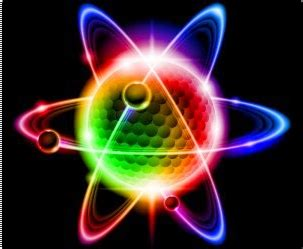
\includegraphics[width=0.8\linewidth]{atome.jpg}
%     \end{figure}
%     \end{frame}

%     \begin{frame}
%         \frametitle{ça?}
        
%         \begin{figure}
%             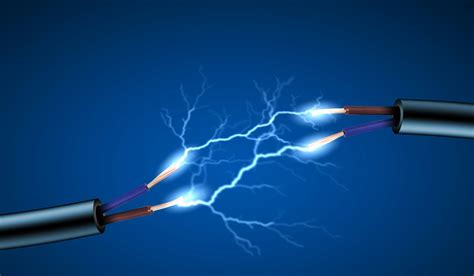
\includegraphics[width=0.8\linewidth]{electricite.jpg}
%     \end{figure}
%     \end{frame}

%     \begin{frame}
%         \frametitle{peut être ça?}
        
%         \begin{figure}
%             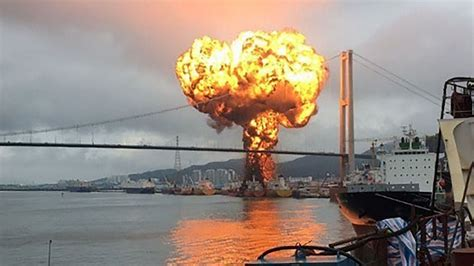
\includegraphics[width=0.8\linewidth]{explosion.jpg}
%     \end{figure}
%     \end{frame}

%     \begin{frame}
%         \frametitle{ou bien ça?}
        
%         \begin{figure}
%             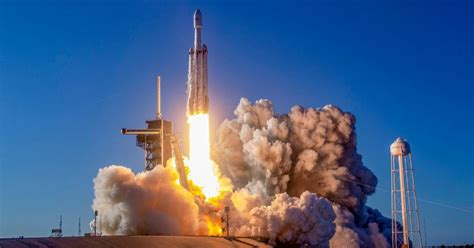
\includegraphics[width=0.8\linewidth]{fusee.jpg}
%     \end{figure}
%     \end{frame}

%     \begin{frame}
%         \frametitle{ou un peu tout ça à la fois...}
        
%         \begin{figure}
%             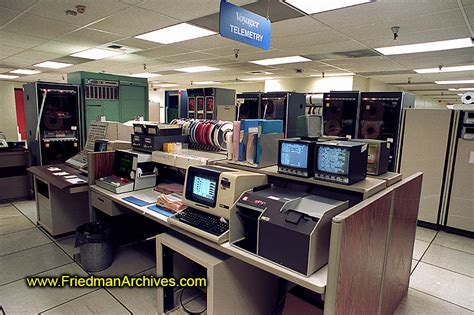
\includegraphics[width=0.8\linewidth]{nasa_computer.jpg}
%     \end{figure}
%     \end{frame}
    

%     \begin{frame}
%         \begin{center}
%             Correction du questionnaire
%         \end{center}
%     \end{frame}

%     \begin{frame}
%         \begin{center}
%             Brainstorming sur qu'est-ce que la physique chimie et à quoi ça sert
%         \end{center}
%     \end{frame}


%     \begin{frame}
%         \frametitle{Les devoirs pour la prochaine fois}
%         \begin{enumerate}
%             \item Faire la page de garde de son cahier ou porte-vues
%             (nom, prénom, matière, année, nom de l'enseignant.e)
%             \item Signer le document : 'bien fonctionner en physique chimie' 
%         \end{enumerate}
%     \end{frame}



% %------------------------------------------------

\begin{frame}
\Huge{\centerline{Fin}}
\end{frame}

%----------------------------------------------------------------------------------------

\end{document} 